\documentclass[border=8pt]{standalone}
\usepackage[scaled=0.95]{helvet}
\renewcommand{\familydefault}{\sfdefault}
\usepackage{tikz}
\usetikzlibrary{arrows.meta,positioning,fit,backgrounds,calc,shapes.geometric,shapes.misc}
\definecolor{ink}{HTML}{16264A}
\definecolor{inksoft}{HTML}{3B4C70}
\definecolor{slate}{HTML}{5D6B7E}
\definecolor{paper}{HTML}{EEF3F1}
\definecolor{rule}{HTML}{C9D6D1}
\definecolor{leaf}{HTML}{1F8A5B}
\definecolor{leafw}{HTML}{E3F3EA}
\definecolor{tur}{HTML}{D98F1C}
\definecolor{turw}{HTML}{FCF0D9}
\definecolor{chilli}{HTML}{C9342B}
\definecolor{chilliw}{HTML}{FBE5E2}
\tikzset{
  >={Stealth[length=2.2mm]},
  box/.style={draw=ink, line width=0.6pt, rounded corners=2pt, fill=white, align=center, inner sep=4pt, font=\small},
  mod/.style={box, minimum width=3.1cm, minimum height=8mm},
  lane/.style={draw=rule, line width=0.8pt, rounded corners=6pt, fill=paper, inner sep=8pt},
  lanetitle/.style={font=\small\bfseries, text=ink, anchor=north west},
  flow/.style={->, line width=0.8pt, draw=ink},
  opt/.style={->, line width=0.8pt, draw=slate, dashed},
  lab/.style={font=\scriptsize, text=slate, fill=white, inner sep=1.5pt},
  ex/.style={font=\scriptsize\itshape, text=inksoft, align=center},
}

\tikzset{
  st/.style={draw=ink, line width=0.9pt, rounded corners=9pt, fill=white, minimum width=3cm, minimum height=11mm, align=center, font=\small\bfseries},
  e/.style={->, line width=0.8pt, draw=ink},
  t/.style={font=\scriptsize, text=inksoft, fill=white, inner sep=1.5pt, align=center},
}
\begin{document}
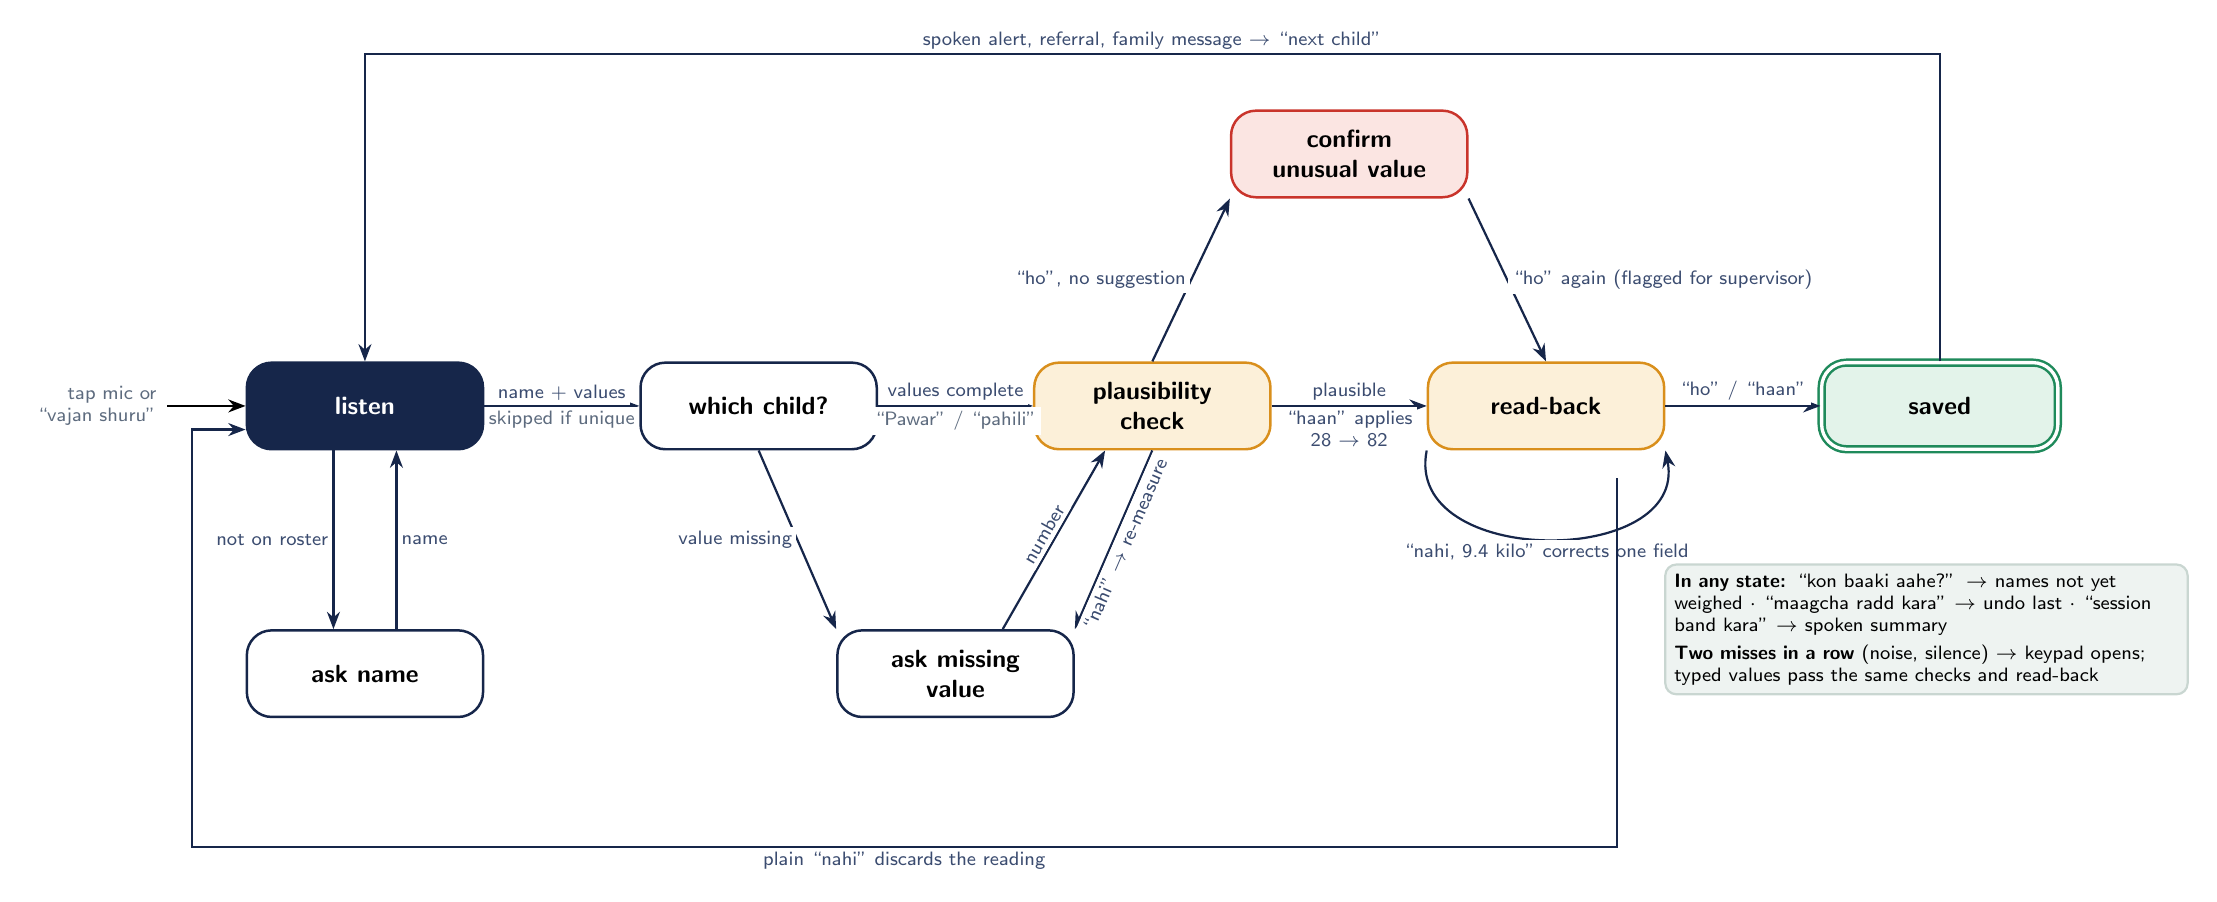
\begin{tikzpicture}
% main path
\node[st, fill=ink, text=white] (listen) at (0,0) {listen};
\node[st] (dis) at (5,0) {which child?};
\node[st, fill=turw, draw=tur] (pl) at (10,0) {plausibility\\check};
\node[st, fill=turw, draw=tur] (conf) at (15,0) {read-back};
\node[st, fill=leafw, draw=leaf, double, double distance=1.2pt] (saved) at (20,0) {saved};
% side states
\node[st] (name) at (0,-3.4) {ask name};
\node[st] (field) at (7.5,-3.4) {ask missing\\value};
\node[st, fill=chilliw, draw=chilli] (force) at (12.5,3.2) {confirm\\unusual value};

\draw[<-, line width=0.8pt] (listen.west) -- ++(-1,0) node[left, font=\scriptsize, text=slate, align=right] {tap mic or\\``vajan shuru''};

\draw[e] (listen) -- node[t, above] {name + values} node[t, below, text=slate] {skipped if unique} (dis);
\draw[e] (dis) -- node[t, above] {values complete} node[t, below, text=slate] {``Pawar'' / ``pahili''} (pl);
\draw[e] (pl) -- node[t, above] {plausible} node[t, below, align=center] {``haan'' applies\\28 $\to$ 82} (conf);
\draw[e] (conf) -- node[t, above] {``ho'' / ``haan''} (saved);

\draw[e] ([xshift=-4mm]listen.south) -- node[t, left] {not on roster} ([xshift=-4mm]name.north);
\draw[e] ([xshift=4mm]name.north) -- node[t, right] {name} ([xshift=4mm]listen.south);
\draw[e] (dis.south) -- node[t, left] {value missing} (field.north west);
\draw[e] ([xshift=6mm]field.north) -- node[t, sloped, above] {number} ([xshift=-6mm]pl.south);
\draw[e] (pl.south) -- node[t, sloped, below] {``nahi'' $\to$ re-measure} (field.north east);
\draw[e] (pl.north) -- node[t, left] {``ho'', no suggestion} (force.south west);
\draw[e] (force.south east) -- node[t, right] {``ho'' again (flagged for supervisor)} (conf.north);

\draw[e] (conf.south west) .. controls +(-0.3,-1.5) and +(0.3,-1.5) .. node[t, below] {``nahi, 9.4 kilo'' corrects one field} (conf.south east);
\draw[e] (saved.north) -- ++(0,3.9) -| node[t, pos=0.25, above] {spoken alert, referral, family message $\to$ ``next child''} (listen.north);
\draw[e] (conf.south) ++(0.9,-0.35) -- (15.9,-5.6) -- node[t, below] {plain ``nahi'' discards the reading} (-2.2,-5.6) |- ([yshift=-3mm]listen.west);

% global commands
\node[draw=rule, line width=0.8pt, rounded corners=4pt, fill=paper, align=left, font=\scriptsize, anchor=north west, text width=6.4cm] at (16.5,-2.0) {
\textbf{In any state:} ``kon baaki aahe?'' $\to$ names not yet weighed $\cdot$ ``maagcha radd kara'' $\to$ undo last $\cdot$ ``session band kara'' $\to$ spoken summary\\[2pt]
\textbf{Two misses in a row} (noise, silence) $\to$ keypad opens; typed values pass the same checks and read-back};
\end{tikzpicture}
\end{document}
